\chapter{Componente tecnologica}
\section{Introduzione}
La realizzazione del progetto prevede, dopo la definizione di una precisa architettura, l'utilizzo di diverse componenti tecnologiche, come ad esempio l'utilizzo di un framework, per soddisfare i vari requisiti utente.
\section{Strumenti utilizzati per l'organizzazione del lavoro}
\subsection{ClickUp}
Ai fini di organizzare per il meglio il lavoro da svolgere, l'utilizzo della piattaforma ClickUp ha permesso al team di sviluppo la suddivisione dei compiti da svolgere mediante la definizione di macro-task, organizzati in dashboard visibili dal settore amministrativo e tecnico. Un macro-task rappresenta l'implementazione di un caso d'uso utente e corrisponde ad un rilascio in produzione. Inoltre prevede un'univocità all'interno della dashboard ed è visibile e modificabile dal reparto di amministrazione per supervisionare l'andamento del progetto. A sua volta un macro-task è suddiviso in task, i quali sono organizzati nei diversi pannelli (admin, negozio, utente, comune) riprendendo il codice univoco a cui è associato il macro-task. Ogni task è inserito nella dashboard gestita dal team di sviluppo e corrisponde all'implementazione di una micro-funzionalità. Deve soddisfare precisi requisiti, di seguito elencati.
\begin{itemize}
    \item \textbf{Durata Limitata}: un task deve prevedere un tempo di implementazione da una alle quattro ore complessive
    \item \textbf{Atomicità}: un task deve prevedere l'implementazione/correzione di funzionalità singole
    \item \textbf{Univocità}: un task non deve essere mai ripetuto, per implementare bugfixes è necessario creare un nuovo macro-task e di seguito organizzarne la suddivisione
    \item \textbf{Reperibilità}: un task deve essere facilmente trovato ricercando parole chiave definite nel titolo, il quale segue lo standard <<\textit{COD \# - Titolo breve}>>
\end{itemize}
Ogni task nel flusso di lavoro può assumere diversi status:
\begin{itemize}
    \item \textbf{Open}: il task è appena stato creato e non è ancora stato implementato
    \item \textbf{In Progress}: il task è in corso di implementazione da parte del team di sviluppo
    \item \textbf{Review}: il task è in corso di revisione da parte dei preposti al testing
    \item \textbf{Closed}: il task è concluso e testato
\end{itemize} 
Un macro-task può passare nello status "closed" solo quando tutti i task a lui relativi sono in closed. A questo punto è possibile procedere con il rilascio della piattaforma in produzione.
\begin{figure}[!htb]
    \centering
    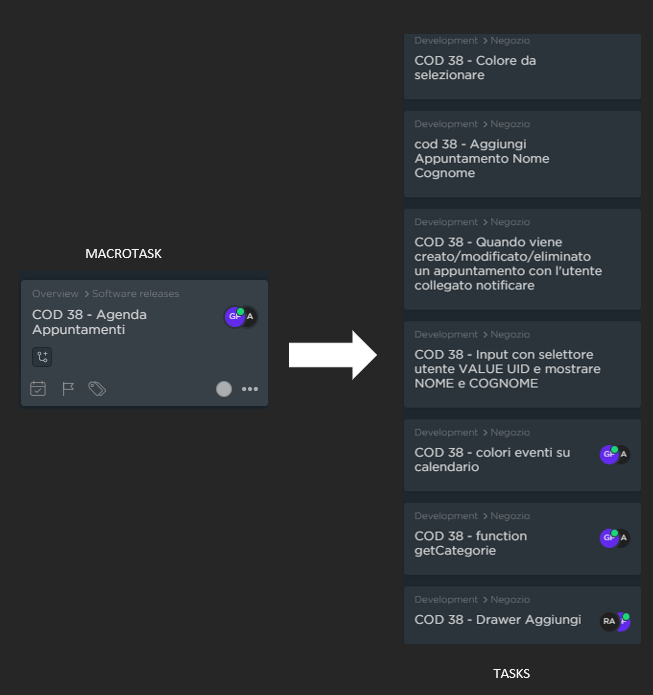
\includegraphics[width=0.7\textwidth]{divis.png}
    \caption{Esempio di organizzazione macrotask - tasks di una funzionalità di Garzone}
\end{figure}
\subsection{Bitbucket}
Per consentire la condivisione ddel codice sorgente tra il team di sviluppo è stato previsto l'utilizzo della piattaforma Bitbucket, un servizio di hosting per progetti implementati tramite utilizzo del protocollo di version control Git. Per l'implemntazione del progetto sono state create quattro apposite repository:
\begin{itemize}
    \item \textbf{garzone-serverless}: la quale comprende tutto il codice sorgente relativo alla componente backend
    \item \textbf{garzone-webapp-admin}: relativo al pannello admin
    \item \textbf{garzone-webapp-negozio}: relativo al pannello negozio
    \item \textbf{garzone-webapp-comune}: relativo al pannello comune
    \item \textbf{garzone-webapp-utente}: relativo al pannello utente
\end{itemize}   
Le operazioni di version control sono state effettuate tramite l'utilizzo di Github Desktop, un'applicazione che utilizza il protocollo Git mediante un'interfaccia grafica. Ad ogni task del progetto implementato è correlato un commit creando quindi un riferimento al flusso di lavoro definito in partenza. 
\subsection{Separazione ambienti di lavoro}
La separazione degli ambienti di lavoro è necessaria per permettere al team di sviluppo di lavorare alle implementazioni di test parallelamente a quelle in produzione. In questo modo si consente un corretto utilizzo della piattaforma da parte dell'utenza su una versione testata e la possibilità da parte degli sviluppatori di procedere con il live deploy solo dopo aver testato il deploy di test. Al progetto vero e proprio firebase-hosted ne è stato quindi affiancato un altro parallelo, il quale presenta lo stesso identificativo \textit{(piattaforma-garzone)} con l'aggiunta del suffisso \textit{"-test"}. I due progetti presentano la medesima suddivisione di sottodomini e si interfacciano a backend differenti, i quali a loro volta si interfacciano a due istanze di basi di dati differenti.
Per l'avvio e la sua messa in produzione, il progetto prevede l'utilizzo di script appositi per ogni pannello, ognuno dei quali ha una funzione specifica di avvio o di deploy. Di seguito vengono proposti gli script relativi alla parte di backend e relativi alla componente frontend del pannello utente, seguiti da una panoramica generale dei servizi a cui si interfacciano le varie piattaforme.
\begin{figure}[!htb]
    \centering
    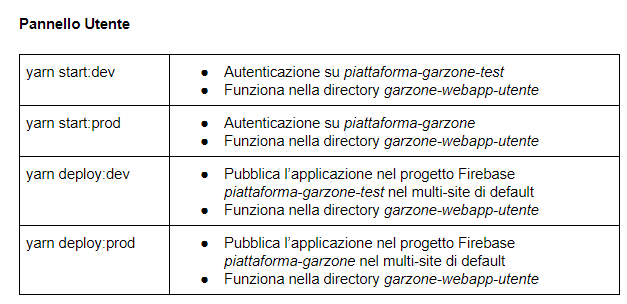
\includegraphics[width=0.8\textwidth]{ut.png}
    \caption{Documentazione degli script di avvio/deploy del pannello utente}
\end{figure}
\begin{figure}[!htb]
    \centering
    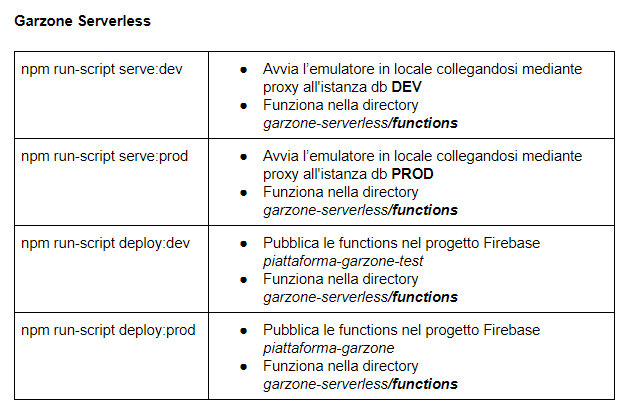
\includegraphics[width=0.8\textwidth]{serv.png}
    \caption{Documentazione degli script di avvio/deploy della componente backend (firebase functions)}
\end{figure}

\begin{figure}[!htb]
    \centering
    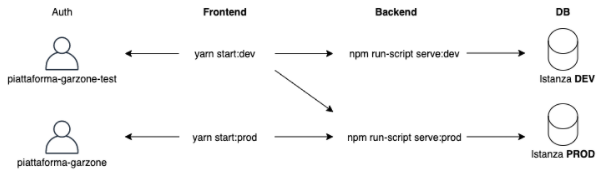
\includegraphics[width=0.8\textwidth]{env.png}
    \caption{Sommario script di avvio dei progetti di test e live e relative interfacce}
\end{figure}
\section{Javascript e NodeJS}
Il progetto è interamente realizzato tramite l'utilizzo del linguaggio Javascript. Fu introdotto nel 1995 come strumento per inserire programmi nelle pagine web del browser Netscape Navigator. Successivamente è stato via via adottato da tutti gli altri browser grafici, rendendo realizzabili moderne applicazioni Web con le quali si può interagire direttamente, senza dover necessariamente ricaricare la pagina. Vie anche utilizzato in siti più tradizionali per offrire varie forme di interattività.\cite{JS}. Node.js è stato creato tramite l'utilizzo di javascript. In particolare si tratta di un ambiente asincrono ed event driven per la costruzione di applicazioni distribuite basate su Javascript. Node.js non è un framework, lavora infatti a livelli più bassi, è sostanzialmente un interprete con alcune librerie di base non native del linguaggio Javascript, ad esempio per l’I/O su file, per l’implementazione di 
server per vari protocolli standard. Sfrutta il loop di gestione degli eventi di Javascript, in particolare sulla possibilità 
di definire funzioni callback per implementare uno schema di I/O non 
bloccante.

\paragraph{Linee guida stesura del codice} Il team di sviluppo per la stesura del codice ha adottato uno standard comune a tutte le sue componenti. La struttura dei file di codice sorgente è stati quindi organizzata in:
\begin{itemize}
    \item \textbf{Screens}: ogni schermata dell'applicazione è rappresentata da un file di codice sorgente in questa directory
    \item \textbf{Components}: ogni componente complesso all'interno di una schermata deve essere inserito in un file di codice sorgente apposito, per consentire una maggiore leggibilità e manutenibilità della soluzione
    \item \textbf{Controllers}: ogni componente dell'UI per interfacciarsi con la logica dell'applicativo comunica con un controller che ha lo scopo di delegare questo compito alla parte di backend
    \item \textbf{Assets}: ogni componente grafica o file di dati statico è organizzato in questa cartella e utilizzato in vari punti del codice
    \item \textbf{Config}: i file di configurazione delle librerie esterne, la validazione dei dati e impostazioni varie, quali palette di colori e stringhe statiche, sono organizzati in questa cartella 
    \item \textbf{Utility}: tutte le funzioni delegate a compiti complessi, come il calcolo del totale dei prezzi degli articoli di un carrello, sono contenute in file in questa directory
    \item \textit{App.js}: rappresenta il codice sorgente radice dell'interfaccia grafica dell'applicazione react
    \item \textit{index.js}: rappresenta il codice sorgente radice dell'applicazione stessa e ha il compito di eseguire l'inizializzazione delle componenti logiche e grafiche, come lo Store di Redux, una libreria di React per la gestione dello stato globale
\end{itemize} 
\begin{figure}
\centering    
\framebox[\textwidth]{%
\begin{minipage}{0.9\textwidth}
\dirtree{%
 .1 {/src} .
  .2 {/Screens} .
  .2 {/Components} .
  .2 {/Controllers} .
  .2 {/Assets} .
  .2 {/Config} .
  .2 {/Utility} .
  .2 {App.js} .
  .2 {index.js} .
}
\end{minipage}
}
\caption{Struttura delle directory e dei file di un pannello di Garzone}
\end{figure}
Inoltre è stato previsto uno stile di stesura ispirato a Airbnb JavaScript\cite{AIRBNB}, che contiene un elenco di best practices per evitare errori di scrittura e con lo scopo di coordinare il metodo di stesura di codice del team di sviluppo.
\subsection{NPM e Yarn}
NPM è un sistema di gestione pacchetti scritti in Javascript in ambiente Node.js. Di norma contengono collezioni di funzioni alcune delle quali esportate, ovvero "visibili" all'esterno del modulo e quindi richiamabili dal progetto. Per la realizzazione di Garzone sono stati utilizzati numerosi pacchetti, con il compito di interfacciarsi a API esterne e realizzare componenti grafiche complesse come ad esempio mappe interattive. Inoltre è stato utilizzato per l'implementazione di script di esecuzione e rilascio dell'applicativo con configurazioni ad hoc. Per le componenti frontend è stato invece utilizzato Yarn, un packet manager costruito a un livello di astrazione superiore di npm, fornendone una semplificazione della sintassi delle istruzioni eseguibili.
\newpage
\section{Componente Frontend}
\subsection{Linee guida grafiche per l'interfaccia utente}
Per la realizzazione delle interfacce grafiche il team di sviluppo ha fatto uso di mockups realizzati dal team grafico. Ogni mockup prevede file generati dal software AdobeXD dai quali è possibile esportare ogni componente grafico (asset) per poi importarlo nel progetto. La progettazione ha previsto l'implementazione di standard condivisi tra i pannelli, ad esempio una palette di colori, il font utilizzato dalla Pubblica Amministrazione su indicazione delle linee guida AGID, le dimensioni di vari componenti e del font, animazioni grafiche e così via. Ogni schermata dell'applicativo prevede quindi una controparte realizzata in AdobeXD.
\subsection{ReactJS}
Il framework su cui si basano le intere interfacce grafiche di Garzone è ReactJS, una libreria JavaScript che mette a disposizione numerose funzionalità logiche e grafiche per ottenere una user experience efficace. L'utilizzo di ReactJS ha messo a disposizione del team di sviluppo numerosi vantaggi, tra cui:
\paragraph{Riutilizzo del codice} ReactJS è una libreria \textbf{component-based}, ovvero permette l'incapsulamento di componenti logico-grafici per l'utilizzo in varie parti dell'applicativo attraverso l'utilizzo delle \textit{<<props>>}.
\paragraph{Manutenibilità del codice} L'incapsulamento dei componenti prevede, tra le altre cose, una maggiore facilità nel manutenere il codice. Infatti è possibile, tramite una singola modifica, modificare lo stesso componente in tutte le parti dell'applicativo.
\paragraph{State management e Virtual DOM} ReactJS prevede che al cambiare delle informazioni (dati) contenute all'interno dello stato di un componente, l'interfaccia grafica venga aggiornata automaticamente con le nuove informazioni contenute nello stato. Questo è reso possibile dall'utilizzo del Virtual DOM, ovvero una rappresentazione del DOM originale della pagina. Al verificarsi di un evento, React occorre le modifiche necessarie sul Virtual DOM e successivamente, dopo l'analisi delle differenze tra Virtual DOM e DOM effettivo, riporta le modifiche sul DOM vero e proprio. Il Virtual DOM è composto quindi da nodi gerarchici chiamati \lstinline[basicstyle=\ttfamily]!ReactNode!, dai quali ereditano anche gli elementi \lstinline[basicstyle=\ttfamily]!ReactElement!, l'elemento più comune in React utilizzato per il rendering di componenti scritti sfruttando il JSX, e \lstinline[basicstyle=\ttfamily]!ReactText!, l'oggetto per il rendering del testo nei nodi del virtual DOM.
\\[12pt]
I componenti in React seguono un ciclo di vita predefinito costituito dai principali eventi \textit{init}, \textit{render} e \textit{mount}.
\paragraph{Inizializzazione} L'inizio del ciclo di vita di un componente React prevede la definizione del suo stato iniziale, ovvero un oggetto JavaScript utilizzato da React per la creazione del Virtual DOM. L'oggetto \textit{<<state>>} creato sarà quindi accessibile dal componente solo dopo la sua inizializzazione.
\paragraph{Rendering} React nella fase di rendring ha il compito di materializzare i nodi contenuti nel componente, facendo uso dello stato creato nella fase di inizializzazione. Il metodo di render viene richiamato ogni qualvolta l'oggetto di stato viene aggiornato ed è richiesto per la definizione di un componente.
\paragraph{Montaggio e Smontaggio} React prevede la possibilità di intercettare la fase di ciclo di vita in cui il componente viene "montato" sulla pagina, ovvero quando la libreria ha concluso il rendering di tutti i nodi contenuti nel componente. Così come esiste la possibilità di intercettare il montaggio, è possibile intercettare anche l'evento di smontaggio del componente, ovvero quando gli elementi del componente facenti parte del DOM vengono rimossi. Di norma per un componente ad una navigazione verso una schermata dell'applicazione esistono una e una sola fase di montaggio e una e una sola fase di smontaggio.
\begin{figure}[!htb]
    \centering
    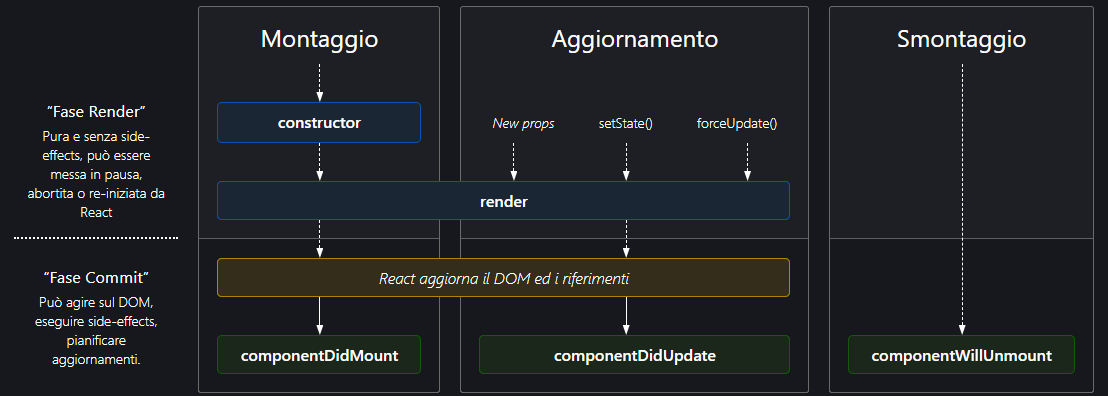
\includegraphics[width=1\textwidth]{lifecycle.png}
    \caption{Ciclo di vita di un React Component\cite{LIFE}}
\end{figure}
\\[12pt]
In React è possbile implementare due tipologie di componenti:
\begin{itemize}
    \item \textbf{Class Components}: estensioni della classe React.Component
    \item \textbf{Function Components}: componenti funzionali basati sulla logica degli \textit{<<hooks>>}, ovvero funzionalità che permettono il riutilizzo dello stato dei componenti nelle varie gerarchie, senza modificarne la logica e permettono una maggiore facilità d'uso riguardo il cilo di vita di un componente
\end{itemize} 
\begin{figure}[!htb]
    \centering
    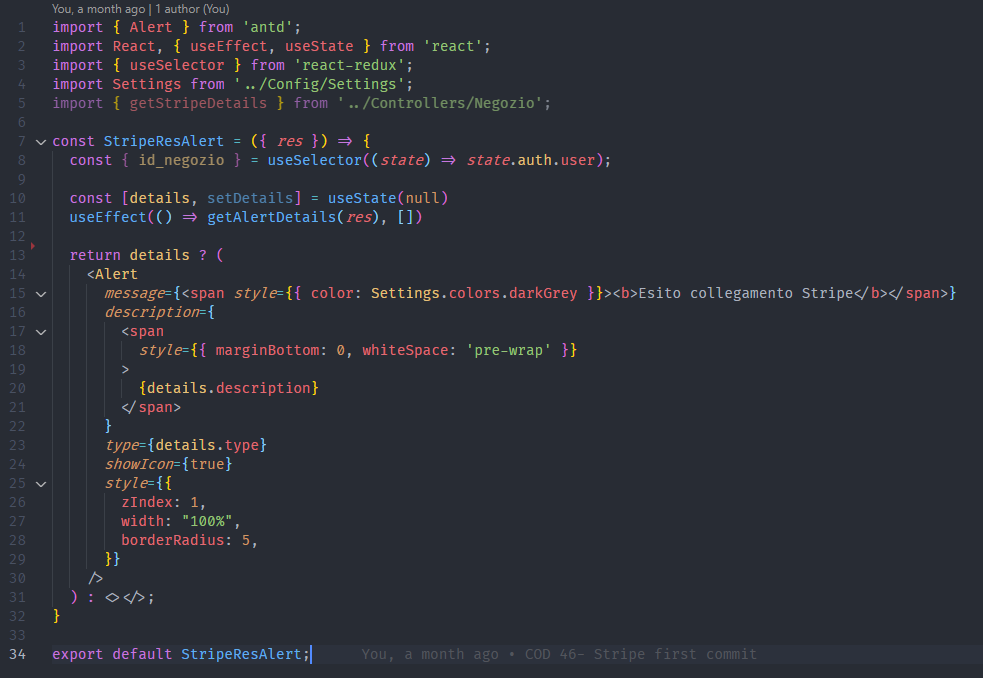
\includegraphics[width=1\textwidth]{func.png}
    \caption{Esempio di Function Component in Garzone}
\end{figure}
\begin{figure}[!htb]
    \centering
    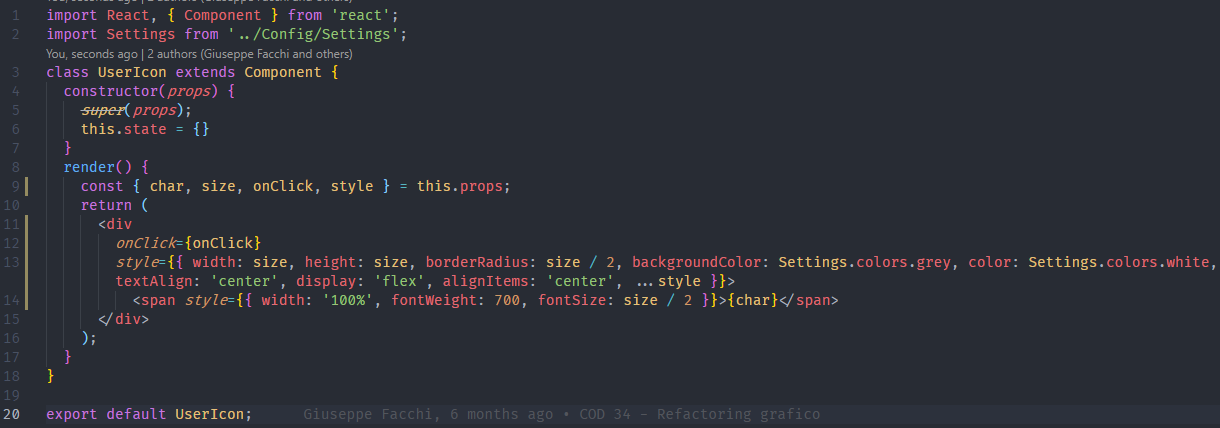
\includegraphics[width=1\textwidth]{class.png}
    \caption{Esempio di Class Component in Garzone}
\end{figure}
\subsection{antd}
Per facilitare l'implementazione dei componenti grafici è stato previsto l'utilizzo del framework grafico \textit{antd}. Creato come libreria UI di React, antd contiene un set di componenti e demo per costruire interfacce grafiche interattive\cite{ANTD}. In Garzone, antd è stato importato tramite l'utilizzo del packet manager Yarn, e ne sono stati implementati i vari moduli facendo uso del tree shaking introdotto in Javascript ES6 con l'istruzione \lstinline[basicstyle=\ttfamily]!import!.
\paragraph{Sovrascrizione stili con Less} Antd offre l'opportunità di sovrascrivere lo stile dei propri componenti utilizzando Less, una libreria che permette di scrivere stili con una sintassi formale e una logica definita. In Garzone sono state sovrascritte gran parte delle variabili di stile implementate da antd e sono stati opportunamente modificati gli script di esecuzione della soluzione, inserendo e utilizzando \lstinline[basicstyle=\ttfamily]!craco! \textit{(Create React App Configuration Override)}: un layer sovrastante il packet manager che offre la possibilità di aggiungere configurazioni particolari alla soluzione. 
\newpage
\section{Componente Backend}
\subsection{Google Cloud}
La realizzazione della componente backend ha previsto un'interfaccia all'ecosistema Google Cloud che, tra le altre cose, mette a disposizione un ambiente di hosting, un ambiente FaaS (Function as a Service), un servizio completamente gestito per database relazionali e altri tool di sviluppo e documentazione come Google Workspace. \\ Per la realizzazione di Garzone sono stati creati due progetti Google Cloud separati
\begin{itemize}
    \item \textbf{garzone-test}: per l'ambiente di test
    \item \textbf{garzone}: per l'ambiente di produzione
\end{itemize} 
ognuno dei quali si interfaccia a micro-servizi indipendenti sia interni che esterni all'ambiente Google Cloud. Ogni componente del team di sviluppo ha un'utenza collegata al progetto con i privilegi impostati sulle mansioni affidate per la realizzazione del progetto e sono previste stringenti regole di sicurezza per monitorare gli accessi a credenziali e pannelli di amminsitrazione. 
\subsubsection{Cloud SQL}
Cloud SQL, è un servizio completamente gestito per l'hosting di database relazionali come mySql, PostgreSQL e SQL Server. A differenza di soluzioni in-house, offre costi di manutenzione contenuti, continuità aziendale, scalabilità in base al consumo e regole di sicurezza e conformità sempre aggiornate. In Garzone la connessione alla base di dati è prevista solo dalla componente FaaS in due modi:
\begin{itemize}
    \item \textbf{Localmente}: la connessione al servizio avviene dalla sorgente FaaS mediante l'interfaccia dell'emulatore in locale alla base di dati tramite un auth proxy fornito da Google Cloud in fase di setup dell'ambiente 
    \begin{figure}[!htb]
        \centering
        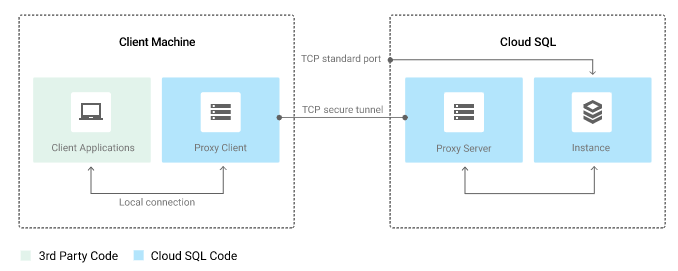
\includegraphics[width=0.7\textwidth]{proxy.png}
        \caption{Connessione da emulatore FaaS a isitanza CloudSQL}
    \end{figure}
    \item \textbf{Da remoto}: la connessione al servizio avviene dalla sorgente FaaS presente sull'host remoto
\end{itemize}
La configurazione della connessione è estratta dalle variabili d'ambiente impostate nel progetto di backend e prevede i seguenti parametri:
\begin{itemize}
    \item \textit{Host}: \lstinline[basicstyle=\ttfamily]!localhost! (solo locale), rappresenta l'host a cui effettuare il collegamento al servizio di CloudSQL
    \item \textit{Port}: \lstinline[basicstyle=\ttfamily]!3306! (solo locale), rappresenta la porta del collegamento
    \item \textit{User}: rappresenta l'utenza per l'autenticazione della connessione all'istanza
    \item \textit{Password}: rappresenta la password per l'autenticazione della connessione all'istanza
    \item \textit{Database}: rappresenta il nome del database a cui collegarsi
    \item \textit{Socket Path}: rappresenta il path dell'istanza  
\end{itemize} 
Per un'ulteriore gestione della base di dati è stato utilizzato il software MySql Workbench, il quale fornisce un'interfaccia grafica interattiva per eseguire operazioni su database. 
\subsection{Firebase}
Firebase è un servizio BaaS (Backend-as-a-service) che consente lo sviluppo di applicazioni offrendo la possibilità di implementare numerose funzioni. I servizi offerti si suddividono in tre macro-categorie\cite{FIRE}:
\begin{itemize}
    \item \textbf{Build}
    \begin{itemize}
        \item \textbf{Realtime Database}: utilizzato per le funzionalità di gestione ordini e chat realtime
        \item \textbf{Authentication}: utilizzata per la fase di login, registrazione e gestione degli utenti
        \item \textbf{Hosting}: utilizzato per il servizio hosting delle piattaforme web
        \item \textbf{Cloud Storage}: utilizzato per l'upload di immagini da parte dell'utenza
        \item \textbf{Cloud Functions}: utilizzate per la parte logica degli applicativi e interfacciarsi alla base di dati
    \end{itemize}
    \item \textbf{Release and Monitor}
    \begin{itemize}
        \item \textbf{Performance e Monitoring}: utilizzati per la gestione degli errori
    \end{itemize}
    \item \textbf{Engage}
    \begin{itemize}
        \item \textbf{Analytics}: servizio utilizzato per visionare il traffico e azioni dell'utenza per poi tracciare strategie di engagement
    \end{itemize}
\end{itemize} 
Firebase offre una console di amministrazione che riprende alcune delle funzionalità offerte da quella di Google Cloud, semplificandone l'interpretazione e l'utilizzo. L'ecosistema Google permette quindi di interfacciarsi direttamente alla soluzione sia da Firebase che dalla piattaforma Google Cloud.
\subsubsection{Firebase Authentication}
La gestione delle utenze in Garzone è delegata a Firebase Authentication, un servizio della suite Google che mette a disposizione un SDK utilizzabile sia dalla componente frontend, sia dalla componente backend. 
\subsubsection{Firebase Functions}
La componente backend dell'applicativo è realizzata tramite l'implementazione delle Firebase Functions, endpoint creati utilizzando un framework serverless che eseguono codice in risposta ad eventi scatenati da altri prodotti Firebase o eventi HTTP. Il ciclo di vita di una cloud function prevede:
\begin{enumerate}
    \item Stesura del codice e configurazione dei parametri di esecuzione
    \item Deploy (rilascio) della funzione
    \item Trigger dell'evento con invocazione ed esecuzione del codice
    \item Se la funzione sta già gestendo numerosi eventi, Firebase crea altre istanze della function velocizzando l'esecuzione complessiva della richiesta
\end{enumerate}
\newpage
In Garzone il codice sorgente delle Firebase Functions presenta una suddivisione in base ai claim dell'utenza. Ad ogni file di functions corrisponde un attore dell'applicativo.
\begin{figure}[!htb]
    \centering    
    \framebox[\textwidth]{%
    \begin{minipage}{1\textwidth}
    \dirtree{%
     .1 {/functions} .
      .2 {/Config} .
      .2 {/Groups} .
        .3 {admin.js} .
        .3 {comune.js} .
        .3 {negozio.js} .
        .3 {utente.js} .
        .3 {general.js} .
      .2 {/Utility} .
    }
    \end{minipage}
    }
    \caption{Struttura delle directory e dei file delle Firebase Functions di Garzone}
\end{figure}
\\Ogni Firebase Function prevede una parte di autenticazione tramite l'utilizzo del \textit{context}, un parametro messo a disposizione in ogni funzione che fornisce informazioni riguardo la provenienza della richiesta. Inoltre prevede una parte di validazione dei dati proveniente dalla richiesta e infine l'esecuzione di codice in base alla funzionalità richiesta. Di seguito un esempio dell'implementazione di una Firebase Function per l'aggiornamento dei campi di un record su database.
\\[12pt]
\begin{lstlisting}[language=JavaScript]
    exports.aggiornaModuloOrdini = functions
  .region("europe-west1")
  .https.onCall(async (data, context) => {
    if (!policies.isProprietario(context, data.id)) {
      throw new functions.https.HttpsError("permission-denied", "Accesso negato");
    } else {
      const aggiornaModuloOrdiniSchema = Yup.object({
        id: Yup.number().required("Id mancante"),
        modulo_ordini: Yup.boolean(),
        ritiro: Yup.boolean(),
        consegna: Yup.boolean(),
        dettagli_consegna: Yup.string()
          .nullable()
          .strict(true)
          .trim("Dettagli consegna con spazi vuoti iniziali/finali")
          .max(1500, "Dettagli consegna > 1500 caratteri"),
      });

      //Validazione richiesta
      const { error, value } = aggiornaModuloOrdiniSchema.validate(data);
      if (error) {
        throw new functions.https.HttpsError("invalid-argument", error, {
          dettaglio: "Errore nella validazione dei campi",
        });
      }

      //Destrutturazione richiesta
      const {
        id,
        modulo_ordini,
        ritiro,
        consegna,
        dettagli_consegna,
      } = data;

      //Composizione dati da inserire [campo_db: valore]
      const negozioRecord = {
        modulo_ordini: modulo_ordini,
        ritiro: ritiro,
        consegna: consegna,
        dettagli_consegna: dettagli_consegna,
      };

      //Update del record con i dati della richiesta
      try {
        const pool = await db.connection;
        await pool.query(`UPDATE negozi SET ? WHERE id=?`, [negozioRecord, id]);
      } catch (error) {
        throw new functions.https.HttpsError("failed-precondition", error, {
          dettaglio: "Errore nell'aggiornamento del record su DB",
        });
      }

      return { success: true };
    }
  });
\end{lstlisting}
\newpage
\subsubsection{Realtime Database}
Firebase Realtime Database è un database NoSQL hostato in cloud che permette il salvataggio e la sincronizzazione dei dati condivisi tra gli utenti in tempo reale. In Garzone è stato implementato per la gestione dei servizi di chat e gestione ordini. 
\begin{figure}[h!]
    \centering
    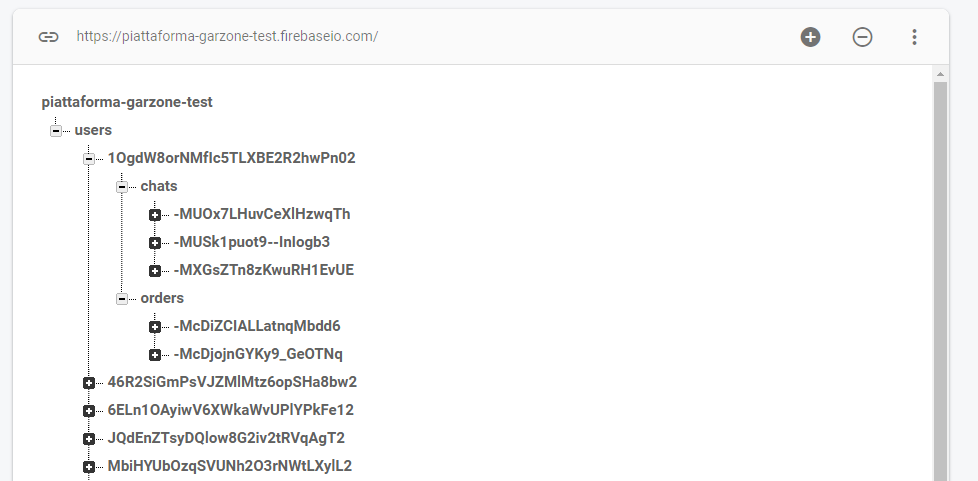
\includegraphics[width=1\textwidth]{rtd.png}
    \caption{Porzione di Firebase Realtime Database in Garzone}
\end{figure}
\FloatBarrier
\subsubsection{Firebase Authentication}
La registrazione, l'accesso e la gestione delle utenze in Garzone sono delegate al servizio di Firebase Authentication, il quale mette a disposizione l'implementazione del suo SDK. Le librerie su cui si basa il servizio sono OAuth 2.0 e OpenID Connect, inoltre Firebase Authentication fornisce servizi di autenticazione di terze parti come Google, Facebook, Twitter e Github, previsti come funzionalità aggiuntive per sviluppi futuri di Garzone. Per l'applicativo è stata inizialmente prevista un'autenticazione tramite mail e password insieme ai servizi di reset. 
\subsubsection{Firebase Cloud Storage}
La gestione delle immagini è affidata al servizio di Firebase Cloud Storage, il quale presenta numerosi vantaggi, tra cui:
\begin{itemize}
  \item Operazioni di download e upload indipendenti dalla qualità di rete del client che le esegue
  \item Modello di sicurezza per consentire l'accesso ai file solo a utenze autorizzate
  \item Scalabilità
\end{itemize}
Ogni file caricato sulla piattaforma viene depositato nel file system di Google Cloud, chiamato bucket. In Garzone il bucket presenta tre directory: 
\begin{itemize}
  \item \textbf{/categorie}, che contiene le immagini delle categorie merceologiche dei negozi, utilizzabili quando un negozio non fornisce un immagini profilo
  \item \textbf{/comuni}, contenente i loghi dei comuni iscritti a Garzone
  \item \textbf{/negozi}, contenente i loghi e le immagini relative a prodotti, servizi e promozioni di ogni negozio
\end{itemize} 
\begin{figure}[h!]
  \centering
  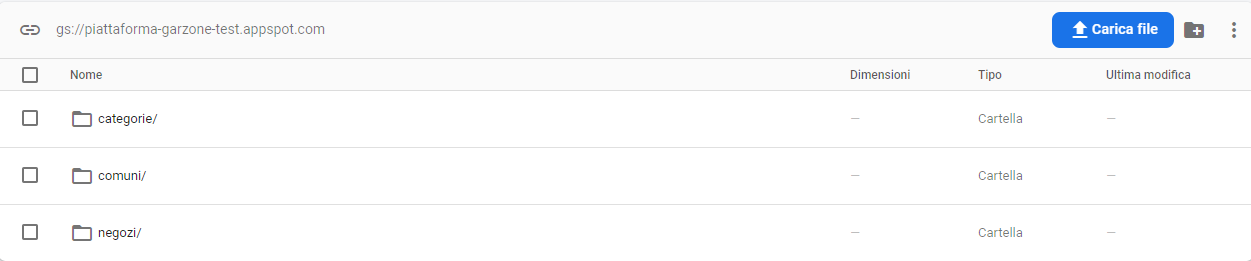
\includegraphics[width=1\textwidth]{bucket.png}
  \caption{Interfaccia grafica console Firebase del Bucket di Garzone}
\end{figure}
\FloatBarrier
\subsection{AWS}
AWS (Amazon Web Services) è un fornitore di servizi web IaaS/PaaS utilizzabili dall'utenza con lo scopo, tra le altre cose, di implementare funzionalità aggiuntive alle proprie soluzioni.
\subsubsection{Simple Email Service} 
In Garzone per lo scambio di e-mail transazionali è stato previsto l'utilizzo del servizio web Simple Email Service. Le opzioni flessibili di distribuzione degli IP e di autenticazione delle e-mail offerte da Amazon SES consentono di incrementare l'efficacia del recapito e di proteggere la reputazione del mittente, mentre le analisi di invio misurano l'impatto di ciascuna e-mail\cite{SES}. Le funzionalità di SES sono state implementate utilizzandone l'SDK nella componente di backend, installandolo tramite il package manager Yarn.
\subsection{Stripe}
Stripe è un servizio web che fornisce prodotti per ricevere pagamenti. In Garzone è previsto l'utilizzo del servizio Stripe \textit{<<Connect>>}, dedicato ai marketplace, ovvero piattaforme intermediarie di vendita tra venditore e consumatore. Stripe fornisce un SDK installabile tramite packet manager Yarn, il quale offre la possibilità di implementare le funzioni per ricevere pagamenti, gestire i payout (pagamenti ai venditori), gestire storni e rimborsi, prevenire frodi e inviare ricevute.
\subsubsection{Stripe Connect}
Connect è un set di strumenti e API programmabili che semplifica i pagamenti sulla tua piattaforma software, la creazione di marketplace e il pagamento di venditori o fornitori di servizi a livello globale, il tutto delegando a Stripe la gestione della conformità dei pagamenti\cite{STRIPE}. Prevede diverse funzionalità necessarie per il funzionamento di un marketplace, come Garzone
\begin{itemize}
  \item Attivazione e verifica delle utenze (negozi)
  \item Accettazione dei pagamenti
  \item Invio di pagamenti agli utenti (negozi)
  \item Gestione delle transazioni e sicurezza
\end{itemize}